\documentclass{article}


\usepackage{PRIMEarxiv}

\usepackage[utf8]{inputenc} % allow utf-8 input
\usepackage[T1]{fontenc}    % use 8-bit T1 fonts
\usepackage{hyperref}       % hyperlinks
\usepackage{url}            % simple URL typesetting
\usepackage{booktabs}       % professional-quality tables
\usepackage{amsfonts}       % blackboard math symbols
\usepackage{nicefrac}       % compact symbols for 1/2, etc.
\usepackage{microtype}      % microtypography
\usepackage{siunitx}
\usepackage{hyperref}
\usepackage{ragged2e}
\sisetup{per-mode=symbol}
\usepackage{lipsum}
\usepackage{parskip}
\usepackage{tabularx}
\usepackage{fancyhdr}       % header
\usepackage{graphicx}       % graphics
\graphicspath{{images/}}     % organize your images and other figures under media/ folder

%Header
\pagestyle{fancy}
\thispagestyle{empty}
\rhead{ \textit{ }} 

% Update your Headers here
\fancyhead[LO]{Aim Is All You Need}
% \fancyhead[RE]{Firstauthor and Secondauthor} % Firstauthor et al. if more than 2 - must use \documentclass[twoside]{article}



  
%% Title
\title{Aim Is All You Need}

\author{
  Seth Katz \\
  \texttt{\{katzseth22202@gmail.com} \\
}

\newcolumntype{L}{>{\RaggedRight\arraybackslash}X}
\newcolumntype{C}{>{\RaggedRight\arraybackslash}c}
\begin{document}
\maketitle

\begin{abstract}\label{sec:abstract}
 In 2017, Google Research published ``Attention is All You Need" \cite{vaswani2023attentionneed}.  Their paper introduced the Transformer, which let neural networks capture long range dependencies.   Just a few years later, OpenAI developed tools like ChatGPT \cite{chatgpt} that resemble hypothetical early prototypes of the computers in Star Trek \cite{startrek}.

But here's the bittersweet truth:  While our screens flicker with progress, the tangible realms of space, energy and paleontology remain comparatively stagnant.

\textbf{Dude, Where's my spaceeship?}

This paper's goal is to enable our progress in physical realms to catch up with our progress online.  Our journey requires applying a single unifying idea that is much simpler than attention - aim.   \begin{figure}[htpb]
    \centering
    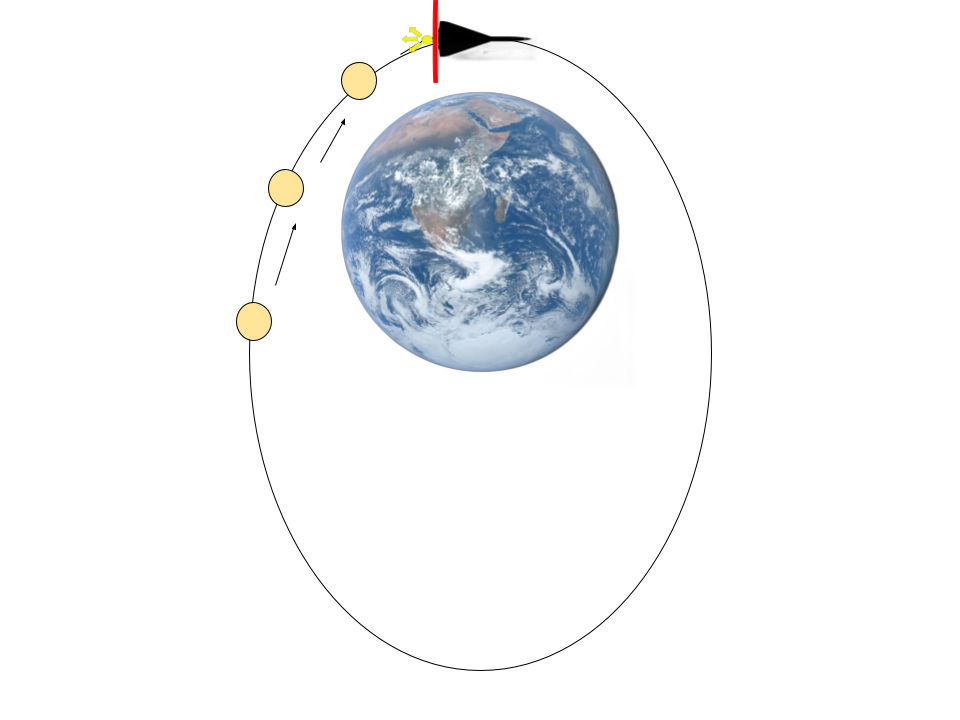
\includegraphics[width=0.5\linewidth]{images/Starship_Impact_ellipse.png}
    \caption{Balloons from a first rocket (not shown) crash into a second target rocket and provide propulsion \cite{earth_image}}
    \label{fig:balloon_impact}
\end{figure}

Consider two rockets.   The first deploys a series of fast moving low density balloons with miniaturized rockets capable of small navigation adjustments.  As shown in \autoref{fig:balloon_impact} these balloons precisely follow a path to sequentially crash  into a separate  target rocket.   These precise collisions deliver high-density jolts of pulsed energy and momentum to the target vehicle, enabling a surprisingly broad range of groundbreaking applications (See \autoref{tab:applications}).    

Paralleling their role in consumer AI, neural networks offer a promising avenue to extend current CubeSat formation flying algorithms with the precise control required for externally pulsed propulsion.

\begin{table}[!htpb]
    \centering
    \caption{A Checklist of Grand Challenges Externally Pulsed Propulsion Can Solve}
    \label{tab:applications}
    \begin{tabularx}{\textwidth}{|c|L|}\hline 
        \textbf{Suborbital Transit} & We'll create a viable suborbital travel vehicle allowing passengers to take off from normal airport runways and reach anywhere in the world in less than 2 hours. Noise pollution near population centers will be no worse than it is with conventional aircraft.\\\hline
        \textbf{Rocket Revolution} & We'll end the tyranny of the rocket equation. We'll still use small rockets, but giant rockets with high propellant mass fraction will no longer be needed to reach orbit.\\\hline
        \textbf{Lunar Lift-off} & Launching from the moon may still require volatiles, but not the more difficult task of making and storing high performance rocket fuel.\\ \hline
        \textbf{Jurassic Dark} & As a side effect of our advances, we'll create the field of lunar paleontology and discover concrete evidence for how life originated on Earth. We'll build a genetic record of extinct species from ancient geological periods, like the dinosaurs. \\\hline
        \textbf{Straw Ways to Heaven} & We can construct terrestrial megastructures, extending from the ground to the edge of space, without relying on advanced magnetic technologies such as Lofstrom Launch Loops \cite{lofstrom_loop}. A particularly ambitious yet beneficial example might be a vacuum tube connecting Earth and space, a "Straw Way to Heaven."\\\hline
        \textbf{Carbon Cancelled} & We will solve our energy problems with carbon negative fuel that absorbs the carbon dioxide produced by industry, all while using minimal land and resources\\\hline
        \textbf{Moon mining} & We'll develop in-situ resource utilization (ISRU) technology, first on our moon and then on icy moons like Saturn's moon Phoebe\\\hline
    \end{tabularx}
\end{table}

Note, this paper summarizes some of the ideas in the blog ``Aim Is All You Need"\cite{aim2024}.
\end{abstract}

\section{Introduction}
Project Orion, conceived in the 1950s, remains the sole propulsion method based on mature contemporary technology that simultaneously offers both specific impulse and thrust superior to chemical rockets\cite{projorion}. Its mechanism involved propelling a spacecraft by directing hypervelocity plasma from nuclear explosions onto a pusher plate. Despite its theoretical promise, Orion faced insurmountable challenges related to political feasibility, radioactive fallout, and the impractical mass requirements stemming from the high minimum yield of nuclear explosions. Nevertheless, Orion conceptually validated the physics of hypervelocity pulsed propulsion.

Our approach replaces nuclear bombs with precisely aimed, hypervelocity gas balloons sequentially impacting a rocket's pusher plate. These balloons can be downscaled to practical sizes.  Unlike nuclear explosions, small hypervelocity gas impacts could be efficiently contained within a pulsed reaction chamber.

Leveraging gravity assists and the Oberth effect \cite{oberth_effect}, hypervelocity balloons could achieve energy densities and specific impulses comparable to Project Orion. This approach wouldn't demand nuclear or massive photovoltaic power, and it would enable lunar launches that use polar volatiles directly without needing to produce rocket fuel.     

Recent cube sat formation flying navigation algorithms and neural network advancements raise the probability of achieving the extremely precise navigation for externally pulsed propulsion.

\section{Externally Pulsed Propulsion  Fundamentals}
To lay the groundwork for understanding the applications of externally pulsed propulsion referenced in \autoref{tab:applications}, let's sketch out some conceptual details. This paper presents a preliminary "back-of-the-envelope" analysis, intended to establish the concept's potential. More rigorous, high-fidelity analyses are reserved for future work.
\subsection{Mass Fraction of Balloon to Rocket Mass}
For externally pulsed propulsion to be a viable option, the ratio of balloon propulsion mass to rocket mass must be low for relevant rocket velocity changes. We develop a closed-form approximation for this ratio ( \autoref{eq:balloon_ratio} in {\autoref{sec:balloon_ratio_approximation}). Since real collisions are not perfectly elastic, our approximation includes an energy loss "fudge factor," \(e\).  Justification for a high \(e\) comes from Project Orion's findings\cite{orion_reflections}.   The Orion team found that pusher plate collisions could be opaque. This opacity implied minimal kinetic energy loss to pusher plate heating, resulting in a more elastic impact. Additionally, a curved, roughly parabolic pusher plate would produce a  highly collimated gas reflection. Therefore, we select a relatively high  \(e=0.8\).   

Relevant mass ratios and mission scenarios are summarized in \autoref{tab:mass_scenarios}. This table clearly shows that externally pulsed propulsion can lift significant mass into orbit. For instance, if a reusable rocket like SpaceX Starship \cite{starship} could launch 25 tons of balloons into a trans-lunar orbit, they then propel a 32 ton rocket into low Earth orbit. This exceeds the Space Shuttle's maximum capacity \cite{space_shuttle_program} or the Zero Fuel Mass of smaller regional jets like the Embraer E170 \cite{embraer_e170}.



\begin{table}[!htpb] % tabularx should be inside a table environment
    \centering
    \caption{Mass Ratio of balloon to rocket with fudge factor \(e=0.8\)}
    \label{tab:mass_scenarios}
    \begin{tabularx}{\textwidth}{|c|c|c|c|L|}\hline % Remove the extra { on this line
        \textbf{\(v_{rf}\) (\SI{}{\km\per\second})} & \textbf{\(v_b\) (\SI{}{\km\per\second})} & \textbf{\(v_{ri}\) (\SI{}{\km\per\second})} & \textbf{\(\frac{m_r}{m_b}\)} & \textbf{Scenario} \\\hline
        7.784 & 10.916 & 0 & 1.28 & Eccentric balloons with apogee at lunar distance pushes rocket to minimal low Earth orbit\\\hline
        0 & 7.784 & 7.784 & 2.308 & Decelerate intercity rocket for powered reentry with retrograde balloons in low orbit \\\hline
        0 & 10.916 & 7.784 & 2.97 & Decelerate intercity rocket for powered reentry with retrograde balloons from lunar orbit \\\hline
        21.518 & 69.277 & 0 & 4.30 & Balloons approach Earth from Jupiter retrograde Hohmann trajectory and push the object to escape velocity and then to a periapsis near Parker Space probe \\\hline
        42.673 & 69.277 & 0 & 1.671 & Balloons approach Earth from Jupiter retrograde Hohmann trajectory and push the object to escape velocity and then to a periapsis near Parker Space probe \\\hline
        3 & 6.421 & 0 & 2.54 & Launch balloons from the moon to trans-lunar injection orbit with low periapsis on Earth \\\hline
        0 & 2.58 & 2.38 & 2.17 & Decelerate trans-lunar payloads to land on the moon \\\hline
    \end{tabularx}
\end{table}


\section{To the moon by water balloon.  Reaching Orbit with External Pulsed Propulsion}
Before we delve into the engineering details of external pulsed propulsion, let's consider how it could significantly enhance the utility and appeal of giant reusable rockets like SpaceX's Starship \cite{starship}.   
\subsection{Making Starship's excess capacity useful to satellite customers}
SpaceX's Starship may be the first fully reusable rocket. At scale, this could dramatically reduce space flight costs.   However, the rocket's large payload size is probably too big for today's space industry needs. For example, in \textit{The New York Times}
\begin{quote}
Carissa Christensen, the chief executive of Bryce Tech, an analytics firm that tracks the launch market, says launching Starship frequently will be key to closing SpaceX’s business case, but finding customers to fill the rocket’s giant payload capacity will be challenging. 
"Starship's payload capacity is huge; it's very, very big, and there aren't that many commercial uses today for a rocket that big," she said.  "Maybe it'll be so cheap that it makes sense to launch satellites on it if its not full or near full."  \cite{nyt_starship_size}
\end{quote}
Although many satellites might be too small to fill up Starship, they can still be very expensive to build and test. For an extreme example, the James Webb Telescope \cite{james_webb_space_telescope} cost \$9.7 billion dollars \cite{jwst_cost} to build. \textit{McKinsey Consulting} argues 
\begin{quote}
Safety and reliability will continue to be overarching concerns, suggesting excellent execution will be table stakes for a competitive launch company. \cite{mckinsey_reliability}
\end{quote}
Once rockets start ferrying astronauts, reliability becomes even more emphatically non-negotiable. Fully stacked, Starship weighs 5,000 tons at launch \cite{starship}, yet its empty mass is only 300 tons. That’s an awfully thin soda can to entrust with billion-dollar satellites or human passengers.

By contrast, a suborbital rocket that merely reaches 200 kilometers in altitude might have a propellant mass fraction under 50 percent. This greater structural margin allows for more robust, reliable engines and extensive payload protection systems. Of course, such a suborbital rocket cannot reach orbit on its own.  It needs Starship to "push" it with externally pulsed propulsion.
\begin{figure}[htpb]
    \centering
    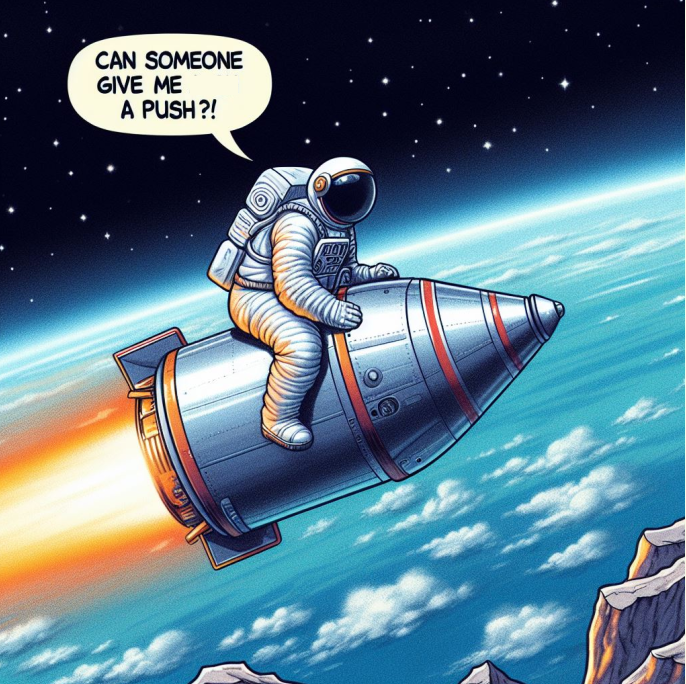
\includegraphics[width=0.5\linewidth]{images/suborbital_push_cartoon.png}
    \caption{A fun and of course very technically accurate cartoon about a suborbital rocket's delta-v limitations}
    \label{fig:suborbital-cartoon}
\end{figure}



Starship launches balloons for externally pulsed propulsion into a highly eccentric orbit around Earth, with a low 200-kilometer perigee and a high apogee. These balloons move near Earth’s escape velocity at perigee. The suborbital rocket intercepts the balloons with its pusher plate and rides their momentum pulses to low Earth orbit. While this approach reduces payload capacity compared to a single rocket system, most satellites are unable to take advantage of Starship’s enormous payload volume anyway.

\subsection{The 200 Mile High Club}
SpaceX proposes direct Earth-to-Earth travel \cite{earth_to_earth}, ballistically launching passengers directly between cities with Starship from offshore platforms. This idea faces significant challenges:
\begin{itemize}
\item Marine environmental impact: Noise pollution from sea launches could severely harm marine ecosystems, including dolphins and whales.
\item Noise over populated areas: Starship's descent would generate loud sonic booms over cities.
\item Logistical inefficiency: Offshore launch platforms, by necessity located far from land, would add hours to the journey for boarding and departure, undermining the benefit of rapid travel.
\end{itemize}
A suborbital rocket plane offers a more practical alternative. To reach orbit, the suborbital rocket requires propulsion balloons launched by the Starship.   Starship can be launched from remote locations where noise pollution is acceptable.  Our suborbital rocket plane could take off from conventional urban airports using standard aircraft engines, then switch to rocket propulsion at high altitudes over remote areas to "skip" above the atmosphere and intercept Starship's propulsion balloons.   While normal airports can handle kerosene or methane fuel, most lack the infrastructure for cryogenic liquid oxygen.

However, two solutions address the liquid oxygen challenge:
\begin{itemize}
\item Air-breathing Scramjets (Optimistic Scenario): If economical passenger scramjets become feasible, rockets could accelerate to around Mach 7 before a steep climb, eliminating the need for liquid oxygen. This would also reduce propellant mass. Unfortunately, the extreme stress on the airframe makes suborbital rockets more economically viable for the foreseeable future.
\item Mid-air oxygen refueling: Suborbital rocket planes could receive liquid oxygen from specialized aircraft launched from airports equipped with liquid oxygen storage. This avoids retrofitting every urban airport, requiring only a single, strategically located airport near major destinations.   Mid-air refueling also reduces our rocket plane's takeoff weight.
\end{itemize}

A formation of propulsion balloons launched in an eccentric Keplerian orbit could only propel the  rocket plane on trajectories that bisect the Earth. Since most urban destinations would not align with such trajectories, the rocket plane needs to fire an adjustment burn at least once to reach the destination.

Alternatively, a second set of propulsion balloons, intercepting the rocket plane mid-flight and adjusting it's trajectory. Furthermore, to avoid a sonic boom upon descent, the plane must decelerate before atmospheric reentry. This deceleration could be provided by yet another set of propulsion balloons that were traveling in a retrograde orbit relative to the plane. Notably, these reentry balloons could be in a circular low Earth orbit rather than a high eccentricity orbit, significantly reducing the mass required.

\section{I Love ISRU.  Cheaper Externally Pulsed Propulsion \textit{Without} Giant Reusable Rockets}
For externally pulsed propulsion to achieve genuine economic competitiveness, the cost of launching its propulsion balloons must be exceptionally low.  The rocket plane must be robust enough to guarantee on-time takeoffs and avoid missing its initial balloon rendezvous. Even highly reusable rockets may prove too expensive, limiting this technology primarily to the very high-end private luxury aviation market. While luxury aviation customers typically prioritize flexibility, balloon-propelled flights necessitate advance scheduling.  Despite these limitations, the potential market for affluent travel between cities like Dubai and Dallas is likely at least an order of magnitude larger than the satellite market.

Still, it would be disappointing if we can't make suborbital travel mainstream.   If we can launch our balloons without giant rockets, we can reduce cost.   After all, "the best part is no part," \cite{best_part_no_part} and a reusable rocket is one heck of a part.

\subsection{Lunar Volatiles for Externally Pulsed Propulsion}

\begin{figure}[htbp]
    \centering
    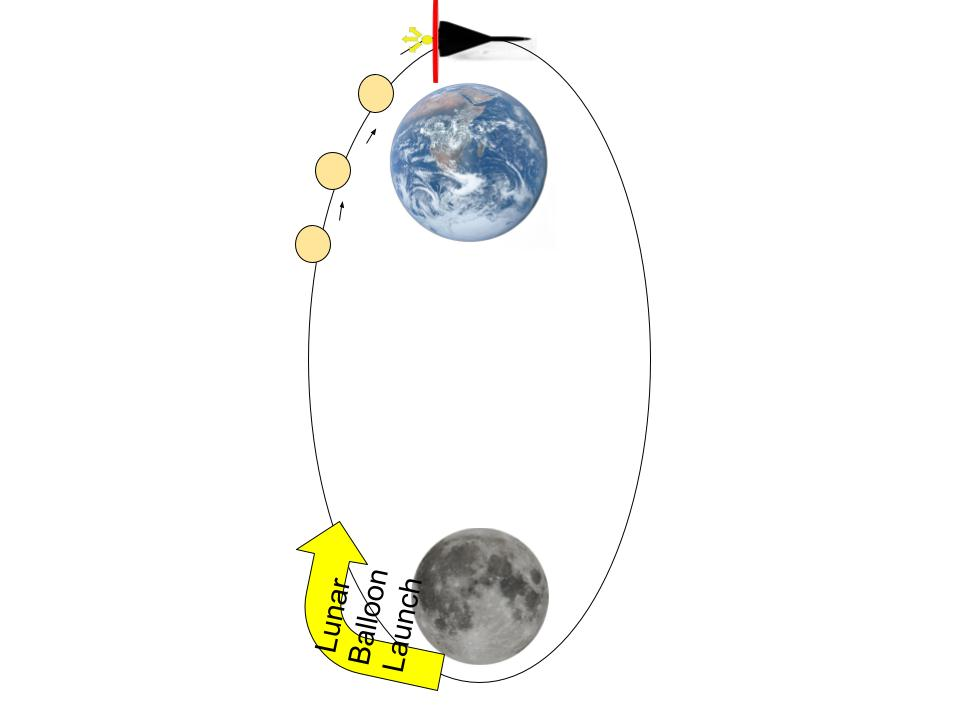
\includegraphics[width=0.5\linewidth]{images/Water Drawing From Moon.jpg}
    \caption{Lunar launched balloons replace Starship launched balloons \cite{earth_image} \cite{moon_image}}
    \label{fig:lunar_launched_balloons}
\end{figure}
Instead of using Starship, lunar volatiles extracted from the moon's permanently shadowed regions could fuel balloons our propulsive balloons. As shown in \autoref{fig:lunar_launched_balloons}, these balloons could be sent into a trans-lunar injection orbit that intersects our terrestrial suborbital rocket plane. Although balloon skins and electronics would likely still be sourced from Earth, volatiles constitute the majority of the balloon's mass. One approach to launching these balloons into orbit involves using rockets powered by lunar-derived propellants. The space community is enthusiastic about water electrolysis to produce and store cryogenic fuel for lunar rockets \cite{nasa_water}. However, this process is energy-intensive and requires complex cryogenic infrastructure, particularly for hydrogen fuel. Moreover, a reusable lunar rocket designed for repeated landings would require approximately \SI{6}{\km\per\second} of delta-v, necessitating propellant mass fractions of about 75\% for hydrogen or 81\% for methane. While these figures are an improvement over Earth-launched rockets, the high propellant mass fractions remain a significant challenge.   

\subsection{Lunar Rockets without Lunar Rocket Fuel}
A clever lunar orbit and externally pulsed propulsion can launch with 
\appendix 
\section{Derivation of Balloon Mass/Rocket Mass Continous Approximation}\label{sec:balloon_ratio_approximation}  We want to approximate the ratio of the total balloon mass \(m_b\) all traveling at velocity \(v_b\) for a sequence of balloons to push a rocket with mass \(m_r\) with initial velocity \(v_{ri}\) to final velocity \(v_{rf}\).   Let's initially naively assume every collision is perfectly elastic in one dimension.   We'll use calculus to get a  closed form expression by solving for a rocket  continously bombarded by infinitestimal balloons each with mass \(dm_b\).   (Note: Grok \cite{grok}  helped with some of the math for this derivation and parts of this derivation are copied from Grok  results directly)

The initial velocities are
\begin{itemize}
\item Mass \( m_r \): Velocity \( v_r \).
\item Balloon: Mass \( dm_b \), velocity \( v_b \).
\end{itemize}
After the collision, let:
\begin{itemize}
    \item Mass \( m_r \): Velocity \( v_r + dv_r \).
    \item Balloon: Velocity \( v_b' \).
\end{itemize}
\subsection{By conservation of momentum} \[
m_r v_r + dm_b v_b = m_r (v_r + dv_r) + dm_b v_b'
\]
\[
m_r v_r + dm_b v_b = m_r v_r + m_r dv_r + dm_b v_b'
\]
\[
dm_b v_b = m_r dv_r + dm_b v_b'
\]
\begin{equation}
m_r dv_r = dm_b (v_b - v_b') \label{eq:momentum}
\end{equation}

\subsection[Velocity change of rocket mass]{Velocity change of \(m_r\)}
For an elastic collision
\begin{equation}
    v_b'\ = \frac{2m_r}{m_r+m_b}v_r + \frac{m_b-m_r}{m_r+m_b}v_b \label{eq:vb_prime_full_momentum}
\end{equation}
Since \(m_r \gg m_b\)   we plug \(m_b = 0\)  into \autoref{eq:vb_prime_full_momentum} and find 
\begin{equation}
v_b' = 2v_r - v_b  \label{eq:vb_prime_result}
\end{equation}      

Substituting \(v_b'\) from  \autoref{eq:vb_prime_result} into \autoref{eq:momentum}:
\[
m_r dv_r = dm_b (v_b - (2 v_r - v_b))
\]
\[
m_r dv_r = dm_b (v_b - 2 v_r + v_b)
\]
\[
m_r dv_r = dm_b (2 v_b - 2 v_r)
\]
\[
m_r dv_r = 2 dm_b (v_b - v_r)
\]
\begin{equation}
dv_r = \frac{2 (v_b - v_r)}{m_r} dm_b \label{eq:vchange_mr}
\end{equation}

\subsection{Integrate over many collisions}
The velocity of \( m_r \) changes from \( v_{ri} \) to \( v_{rf} \) as more balloons collide. Integrate \autoref{eq:vchange_mr}:
\[
\int_{v_{ri}}^{v_{rf}} dv_r = \int_0^{m_b} \frac{2 (v_b - v_r)}{m_r} dm_b
\]
The left-hand side is:
\[
\int_{v_{ri}}^{v_{rf}} dv_r = v_{rf} - v_{ri}
\]
For the right-hand side, treat \( v_r \) as a function of the accumulated balloon mass \( m_b \). However, we need to express \( v_r \) in terms of \( m_b \). From \autoref{eq:vchange_mr}:
\begin{equation}
\frac{dv_r}{v_b - v_r} = \frac{2 dm_b}{m_r}\label{eq:dvr_velocity_relation}
\end{equation}

Since \(v_b\) is constant,  \(dv_b = 0\) and  \(dv_r = -d(v_b-v_r)\), so we can rewrite \autoref{eq:dvr_velocity_relation} as:
\[
-\frac{d(v_b - v_r)}{v_b - v_r} = \frac{2 dm_b}{m_r}
\]
Integrate both sides:
- Left: \( \int_{v_b - v_{ri}}^{v_b - v_{rf}} -\frac{d(v_b - v_r)}{v_b - v_r} = \int_{v_{ri}}^{v_{rf}} \frac{dv_r}{v_b - v_r} \)
\[
= \left[ -\ln|v_b - v_r| \right]_{v_{ri}}^{v_{rf}} = \ln \left| \frac{v_b - v_{ri}}{v_b - v_{rf}} \right|
\]
- Right: \( \int_0^{m_b} \frac{2 dm_b}{m_r} = \frac{2 m_b}{m_r} \)
Equate:
\[
\ln \left| \frac{v_b - v_{ri}}{v_b - v_{rf}} \right| = \frac{2 m_b}{m_r}
\]
Solve for \( m_b \):
\[
\left| \frac{v_b - v_{ri}}{v_b - v_{rf}} \right| = e^{2 m_b / m_r}
\]
\begin{equation}
m_b = \frac{m_r}{2} \ln \left| \frac{v_b - v_{ri}}{v_b - v_{rf}} \right| 
\end{equation}
\subsection{Interpret the Absolute Value}   
The absolute value accounts for the direction of velocities:
- If \( v_b > v_{ri} \) and \( v_b > v_{rf} \),  then \( v_b - v_{ri} \) and \( v_b - v_{rf} \) are positive, so:
\[
m_b = \frac{m_r}{2} \ln \left( \frac{v_b - v_{ri}}{v_b - v_{rf}} \right)
\]
\subsection{Compute Balloon to Rocket Mass Ratio, with a fudge factor for real world losses}

We can then solve for the total balloon to rocket ratio, with a fudge factor e between 0 and 1 to account for the coefficient of restitution and imperfect spread of gaseous volatiles off the pusher plate.   Let's naively assume this fudge factor is the same for each collission even though in practice it would likely vary as the relative velocity of the balloons and the rocket change.
\begin{equation}
\frac{m_r}{m_b} = \frac{2e}{ln(\frac{v_b-v_{ri}}{v_b-v_{rf}})}\label{eq:balloon_ratio}
\end{equation}


%Bibliography
\bibliographystyle{unsrt}  
\bibliography{references}  


\end{document}
